% L10a student companion deck: intrinsic and extrinsic value, the Greeks of
% American options, Delta as a hedge
% ratio and a probability estimate, and the probabilities of exercise and profit.
%
% The frame order mirrors the lecture notebook. The disclaimer is slide 2, by
% instructor preference. Notation follows the lecture: contract type
% \star\in\{c,p\}, premium \mathcal{P}_\star(S,\sigma,t,g_y), Greeks \Delta_\star,
% \Gamma_\star, \Theta_\star, \nu_\star, \rho_\star, signed contract count n, and
% extrinsic value E_V(t). Built October 2026 from the rebuilt lecture (see
% lectures/instructor/L10a-REBUILD-HANDOFF.md). The extrinsic-value figure is the
% extrinsic-value example's SVG converted to PDF with rsvg-convert. October 16,
% 2026: intrinsic and extrinsic value moved here from L9b, after the profile.
% October 20, 2026: Longstaff-Schwartz Monte Carlo (three frames and the example)
% moved here from L9b, right after the profile; lecture-number references removed.
\documentclass[aspectratio=169,11pt]{beamer}
\usepackage{vnslides}

\newcommand{\Pst}{\mathcal{P}_{\star}}
\newcommand{\Q}{\mathbb{Q}}
\newcommand{\PAM}{\mathcal{P}^{\text{AM}}}
\newcommand{\PEU}{\mathcal{P}^{\text{EU}}}
\newcommand{\Dstep}{\mathcal{D}^{-1}_{t+1,t}(g_{y})}
\newcommand{\repo}{https://github.com/varnerlab/CHEME-5660-CourseRepository-Fall-2026/blob/main/lectures/week-10/L10a}

\title{\texorpdfstring{{\vnheavy L10a}}{L10a}: Monte Carlo Pricing and Sensitivity Analysis of American Options Premium}
\subtitle{CHEME 5660 Cornell University}
\author{Copyright Jeffrey Varner 2026. All Rights Reserved}

\begin{document}

\vntitlepage

\begin{frame}{Disclaimer and Risks}
  \vspace{0.6em}
  \textbf{\ink{Training only.}} This content is for training and informational
  purposes only. The teaching team does not make, give, or endorse any offer or
  solicitation to buy or sell securities or derivative products, or provide
  investment or trading advice or strategy.

  \vspace{1.1em}
  \textbf{\ink{Risk.}} Trading involves risk and is generally not recommended for
  those with limited resources, experience, or a low risk tolerance. Past
  performance does not guarantee future success.

  \vspace{1.1em}
  \textbf{\ink{Responsibility.}} You are responsible for your investment decisions
  based on your financial circumstances, objectives, risk tolerance, and
  liquidity needs.
\end{frame}

\begin{frame}{Objectives for Today}
  Previously, we priced American options on a CRR tree. Can simulation price
  them? Duration and convexity measured how a bond's price moves with its yield.
  How much does the premium change when the share price,
  volatility, time to expiration, or interest rate changes?

  \vspace{0.5em}
  {\large\textbf{\ink{Today's concepts}}}
  \begin{itemize}\setlength{\itemsep}{0.4em}
    \item \hilite{Estimate and decompose the premium of American options}:
      Longstaff--Schwartz Monte Carlo, then intrinsic value (immediate exercise
      value) and extrinsic value (time value).
    \item \hilite{Compute the Greeks for American options}: Delta, Theta, Vega,
      Rho, and Gamma from a local Taylor expansion of the options premium.
    \item \hilite{Interpret Delta and compute the probabilities of exercise and
      profit}: the shares needed to hedge an option position, and the
      probabilities from projected share price distributions at the strike
      price and at the breakeven.
  \end{itemize}
\end{frame}

\begin{frame}{Lectures and Examples}
  \vspace{0.3em}
  {\normalsize\textbf{\ink{Lecture:}}\par\small
  \href{\repo/CHEME-5660-L10a-Lecture-American-Derivatives-Greeks-Fall-2026.ipynb}{\dimmed{CHEME-5660-L10a-Lecture-American-Derivatives-Greeks-Fall-2026.ipynb}}}

  \vspace{0.6em}
  {\normalsize\textbf{\ink{Example 1:}}\par\small
  \href{\repo/CHEME-5660-L10a-Example-LSM-Premium-Fall-2026.ipynb}{\dimmed{CHEME-5660-L10a-Example-LSM-Premium-Fall-2026.ipynb}}}

  \vspace{0.45em}
  {\normalsize\textbf{\ink{Example 2:}}\par\small
  \href{\repo/CHEME-5660-L10a-Example-Greeks-PutCall-Fall-2026.ipynb}{\dimmed{CHEME-5660-L10a-Example-Greeks-PutCall-Fall-2026.ipynb}}}

  \vspace{0.45em}
  {\normalsize\textbf{\ink{Example 3:}}\par\small
  \href{\repo/CHEME-5660-L10a-Example-POE-POP-Call-Fall-2026.ipynb}{\dimmed{CHEME-5660-L10a-Example-POE-POP-Call-Fall-2026.ipynb}}}

  \vspace{0.45em}
  {\normalsize\textbf{\ink{Review on your own:}}\par\small
  \href{\repo/CHEME-5660-L10a-Example-ExtrinsicValue-Fall-2026.ipynb}{\dimmed{CHEME-5660-L10a-Example-ExtrinsicValue-Fall-2026.ipynb}}}
\end{frame}

\begin{frame}{Company Profile: Susquehanna}
  \href{https://sig.com/about/}{\hilite{Susquehanna (SIG)}} is a privately held
  trading firm whose core business is options trading. Friends who traded
  options on the floor of the Philadelphia Stock Exchange started it in 1987.
  \begin{itemize}\setlength{\itemsep}{0.35em}
    \item \hilite{Options market making}: it posts prices to buy and sell, so it
      takes the other side of its customers' contracts. In October 2026, it was
      the Designated Primary Market Maker for 1,359 of 5,370 Cboe option
      classes, the most of any firm.
    \item \hilite{Managing the Greeks}: its book is exposed to Delta, Vega,
      Theta, and Rho at once, and the goal is to net these across products.
    \item \hilite{Training}: interns learn options theory, and poker teaches
      new traders to decide under uncertainty.
  \end{itemize}
  \vspace{0.3em}
  \textbf{\ink{Connection to today's lecture:}} when a customer buys a call, the
  firm hedges with $100\,\Delta_{c}$ shares and rebalances as Gamma moves $\Delta_{c}$.
\end{frame}

\begin{frame}{Monte Carlo Pricing of American Options}
  We simulate share price paths under the risk-neutral pricing rule $\Q$, then estimate the value of holding
  at each date by regressing the discounted cash flows from holding on the
  current share price across paths. Like the lattice, Longstaff and Schwartz
  work backward from expiration:

  \vspace{0.6em}
  \hilite{Initialize}: given the share price $S_{0}$, the strike price $K$, the
  payoff function $V(K,S)$ of the call or put, the time to expiration $T$ (years),
  the volatility $\sigma$, the risk-free rate $g_{y}$, the number of exercise dates $h$ after
  today, and the number of paths $M$. Compute $\Delta t=T/h$ and
  $\Dstep=e^{-g_{y}\Delta t}$.
  \slidenote{Reference:}{Longstaff, F. A., and Schwartz, E. S. (2001). Valuing American options by simulation: a simple least-squares approach. \href{https://doi.org/10.1093/rfs/14.1.113}{Review of Financial Studies 14(1): 113–147}.}
\end{frame}

\begin{frame}{Pseudocode: Longstaff–Schwartz}
  \begin{enumerate}\setlength{\itemsep}{0.3em}
    \item \hilite{Simulate}: generate $M$ share price paths under $\Q$ from $S_{0}$
      on the dates $t=0,1,\dots,h$ (expiration), where $S_{i}(t)$ is the share
      price on path $i$ at date $t$.
    \item At expiration, set each path's cash flow to its payoff:
      $Y_{i}(h)\gets V(K,S_{i}(h))$ for $i=1,2,\dots,M$, where $Y_{i}(t)$ is
      path $i$'s cash flow valued at date $t$.
    \item For each date $t=h-1,h-2,\dots,1$ \textbf{do}:
      \begin{itemize}
        \item[a.] Discount each cash flow back one date: $Y_{i}(t)\gets\Dstep\cdot Y_{i}(t+1)$.
        \item[b.] \hilite{Regress}: on the in-the-money paths, those with $V(K,S_{i}(t))>0$, fit the value of holding
          $\hat{C}_{t}(S)=\beta_{0}+\beta_{1}S+\beta_{2}S^{2}$ to the pairs
          $\bigl(S_{i}(t),Y_{i}(t)\bigr)$ by least squares.
        \item[c.] \hilite{Decide}: for each in-the-money path, if
          $V(K,S_{i}(t))>\hat{C}_{t}(S_{i}(t))$, \textbf{then}: exercise, so
          $Y_{i}(t)\gets V(K,S_{i}(t))$.
      \end{itemize}
    \item Discount the cash flows to today and average them:
      $\bar{Y}\gets\mathcal{D}^{-1}_{1,0}(g_{y})\cdot\frac{1}{M}\sum_{i=1}^{M}Y_{i}(1)$.
    \item The premium is $\PAM\gets\max\bigl\{V(K,S_{0}),~\bar{Y}\bigr\}$.
  \end{enumerate}
\end{frame}

\begin{frame}{The Early-Exercise Premium by Simulation}
  Let's price an American put by simulation and compare it with the lattice and
  the European premium. We apply two rules to the same simulated paths:

  \vspace{0.8em}
  \begin{center}
    \begin{tabular}{l@{\hspace{2.5em}}c}
      \toprule
      Rule at each date & Estimates \\
      \midrule
      Longstaff--Schwartz: exercise when $V(K,S_{i}(t))>\hat{C}_{t}(S_{i}(t))$ & $\PAM$ \\[0.2em]
      Hold on every path & $\PEU$ \\
      \bottomrule
    \end{tabular}
  \end{center}
  \begin{equation*}
    \boxed{\text{early-exercise premium}\approx\PAM-\PEU}
  \end{equation*}
  \slidenote{Example 1:}{\href{\repo/CHEME-5660-L10a-Example-LSM-Premium-Fall-2026.ipynb}{\dimmed{CHEME-5660-L10a-Example-LSM-Premium-Fall-2026.ipynb}}}
\end{frame}

\begin{frame}{Extrinsic versus Intrinsic Value}
  The premium (price) of an American option can be broken down into two
  components: intrinsic value and extrinsic value.
  \begin{itemize}\setlength{\itemsep}{0.35em}
    \item \hilite{Intrinsic value}: the immediate exercise value,
      $\max(0, S(t) - K)$ for a call and $\max(0, K - S(t))$ for a put, where
      $S(t)$ is the current share price.
    \item \hilite{Extrinsic value}: also known as time value, the additional
      value from the potential for future price movements before expiration.
  \end{itemize}
  The extrinsic value $E_{V}(t)$ can be expressed mathematically as:
  \begin{equation*}
    \boxed{
    \begin{aligned}
      E_{V}(t) = \text{Option Price} - \text{Intrinsic Value}\quad\blacksquare
    \end{aligned}}
  \end{equation*}
\end{frame}

\begin{frame}{Extrinsic Value}
  In expanded form, the extrinsic value $E_{V}(t)$ is:
  \begin{equation*}
    \boxed{
    \begin{aligned}
      E_{V}(t) &= \begin{cases}
      \mathcal{P}_{c}(K,S(t)) - \max(0, S(t) - K) & \text{(for Call Options)} \\
      \mathcal{P}_{p}(K,S(t)) - \max(0, K - S(t)) & \text{(for Put Options)}
      \end{cases}
    \end{aligned}}
  \end{equation*}
  When the option is \hilite{out of the money}, it has no intrinsic value, and
  the entire option price is extrinsic value.

  \vspace{0.4em}
  \textbf{\ink{Why do people pay money for something that is ``worthless''?}}
  There is still a chance that the share price moves favorably before
  expiration.

  \vspace{0.4em}
  As time moves towards expiration, the extrinsic value tends to decrease
  (\hilite{time decay}), because there is less time for the share price to
  move favorably.
  \slidenote{Review on your own:}{\href{\repo/CHEME-5660-L10a-Example-ExtrinsicValue-Fall-2026.ipynb}{\dimmed{CHEME-5660-L10a-Example-ExtrinsicValue-Fall-2026.ipynb}}}
\end{frame}

\begin{frame}{Call Premium across Strikes and Expirations}
  \vspace{-0.6em}
  \begin{center}
    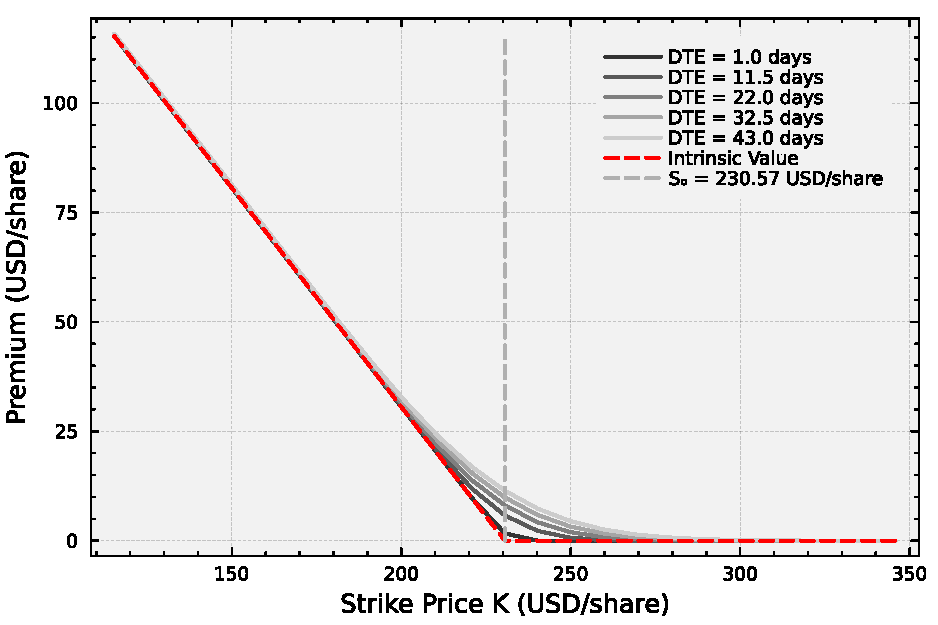
\includegraphics[width=\textwidth,height=0.70\textheight,keepaspectratio]{../figs/CHEME-5660-L10a-Example-ExtrinsicValue-Fall-2026.pdf}
  \end{center}
  \vspace{-0.4em}
  \textbf{\ink{Hmmmm:}} the premium changes with time to expiration and the
  strike price. How does it change with other factors?
\end{frame}

\begin{frame}{The Greeks}
  The \hilite{Greeks} are local sensitivity coefficients that measure how
  American options premiums change with market conditions:
  \begin{itemize}\setlength{\itemsep}{0.35em}
    \item \hilite{Delta $\Delta$}: the change in premium for a
      \texttt{+1~USD/share} change in the share price.
    \item \hilite{Theta $\Theta$}: the change in premium for a
      \texttt{1-day decrease} in the lifetime of the contract (time decay).
    \item \hilite{Vega $\nu$}: the change in premium for a \texttt{+1\%} change
      in volatility.
    \item \hilite{Gamma $\Gamma$}: the change in $\Delta$ for a
      \texttt{+1~USD/share} change in the share price.
    \item \hilite{Rho $\rho$}: the change in premium for a \texttt{+1\%} change
      in the risk-free rate, usually minor except for longer-term options.
  \end{itemize}
  Most trading platforms compute these for you!
\end{frame}

\begin{frame}{A Local Taylor Expansion of the Premium}
  Expanding the premium $\Pst(S,\sigma,t,g_{y})$ of a contract of type
  $\star\in\{c,p\}$ at calendar time $t$ to second order in $S$ and first order in the other inputs:
  \begin{equation*}
    \boxed{
    \begin{aligned}
      \Delta\Pst \approx \Delta_{\star}\,\Delta S + \nu_{\star}\,\Delta\sigma
      + \Theta_{\star}\,\Delta t + \rho_{\star}\,\Delta g_{y}
      + \tfrac{1}{2}\,\Gamma_{\star}\,(\Delta S)^{2}
    \end{aligned}}
  \end{equation*}
  \begin{equation*}
    \Delta_{\star}=\frac{\partial\Pst}{\partial S}\qquad
    \nu_{\star}=\frac{\partial\Pst}{\partial \sigma}\qquad
    \Theta_{\star}=\frac{\partial\Pst}{\partial t}\qquad
    \rho_{\star}=\frac{\partial\Pst}{\partial g_{y}}\qquad
    \Gamma_{\star}=\frac{\partial^{2}\Pst}{\partial S^{2}}
  \end{equation*}
  Derivatives are taken at the current inputs, with $\Delta t$ in years and
  $\Delta\sigma$, $\Delta g_{y}$ in decimals. Platforms quote $\Theta_{\star}/365$ per day, and $\nu_{\star}/100$
  and $\rho_{\star}/100$ per percentage point.
\end{frame}

\begin{frame}{Delta and Gamma as Duration and Convexity}
  $\Delta_{\star}$ and $\Gamma_{\star}$ play the roles of a bond's duration
  and convexity: the slope and the curvature of the premium as a function
  of the share price.

  \vspace{0.5em}
  \textbf{\ink{Example:}} a long call has $\Delta_{c}=0.50$ and
  $\Gamma_{c}=0.02$ per USD/share.
  \begin{align*}
    \Delta S=+5:\quad \Delta\mathcal{P}_{c} &\approx 0.50\times5+\tfrac{1}{2}(0.02)(5)^{2}=2.50+0.25=2.75~\text{USD/share}\\
    \Delta S=-5:\quad \Delta\mathcal{P}_{c} &\approx -2.50+0.25=-2.25~\text{USD/share}
  \end{align*}
  The Gamma term adds to the premium whichever way the share price moves.
\end{frame}

\begin{frame}{Computing the Greeks of American Options}
  Backward induction on the CRR tree gives no formula to differentiate, so we
  reprice the tree with one input moved up and down by a step $\epsilon$:
  \begin{equation*}
    \boxed{
    \begin{aligned}
      \frac{\partial\Pst}{\partial x} & \approx \frac{\Pst(x+\epsilon)-\Pst(x-\epsilon)}{2\epsilon}\qquad x\in\{S,\sigma,t,g_{y}\}\\
      \Gamma_{\star} & \approx \frac{\Pst(S+\epsilon)-2\,\Pst(S)+\Pst(S-\epsilon)}{\epsilon^{2}}
    \end{aligned}}
  \end{equation*}
  With no dividends, a call's American and European premiums are equal,
  so the Black--Scholes--Merton formulas give Greeks to check against,
  e.g., $\Delta_{c}=N(d_{+})$.
  \slidenote{Example 2:}{\href{\repo/CHEME-5660-L10a-Example-Greeks-PutCall-Fall-2026.ipynb}{\dimmed{CHEME-5660-L10a-Example-Greeks-PutCall-Fall-2026.ipynb}}}
\end{frame}

\begin{frame}{The Secret Lives of Delta}
  Besides measuring the premium change for a \texttt{+1~USD/share} move in the
  share price, $\Delta$ has two other interpretations:
  \begin{itemize}\setlength{\itemsep}{0.45em}
    \item \hilite{Hedge ratio}: for every $n$ contracts held ($n<0$ if the
      contracts are sold), hold $-100\cdot n\cdot\Delta$ shares to be
      \hilite{delta-neutral}, i.e., insensitive to small share price moves.
    \item \hilite{Probability of exercise}: $\Delta$ is often used as an
      estimate of the probability that the option expires in-the-money. A call
      with $\Delta=0.7$ suggests a 70\% chance.
  \end{itemize}
\end{frame}

\begin{frame}{Probability of Exercise (POE)}
  The probability that the contract finishes in-the-money at expiration $t=T$:
  \begin{equation*}
    \boxed{
    \begin{aligned}
      \text{POE} & = \begin{cases}
      \mathbb{P}\left(S_{T} > K + 0.01\right) & \text{(for Call Options)} \\
      \mathbb{P}\left(S_{T} < K - 0.01\right) & \text{(for Put Options)}
      \end{cases}
    \end{aligned}}
  \end{equation*}
  where $S_{T}$ is the share price at expiration. In the Black--Scholes--Merton
  model, a European call has
  $\Delta_{c}=N(d_{+})$, while the risk-neutral probability that it finishes
  in-the-money is $N(d_{-})$, which is smaller.

  \vspace{0.5em}
  \textbf{\ink{Conjecture:}} $\Delta\approx\text{POE}$. Example 3 checks it.
\end{frame}

\begin{frame}{Probability of Profit (POP)}
  The probability that the contract's profit at expiration is positive:
  \begin{equation*}
    \boxed{
    \begin{aligned}
      \text{POP} & = \mathbb{P}\left(\hat{P}_{\mathcal{C}} > 0\right)
    \end{aligned}}
  \end{equation*}
  where $\hat{P}_{\mathcal{C}}$ is the profit of the (single or composite)
  contract at expiration.

  \vspace{0.5em}
  POE reads the projected distribution at the strike price, POP at the
  breakeven.
  \slidenote{Example 3:}{\href{\repo/CHEME-5660-L10a-Example-POE-POP-Call-Fall-2026.ipynb}{\dimmed{CHEME-5660-L10a-Example-POE-POP-Call-Fall-2026.ipynb}}}
\end{frame}

\begin{frame}{Optional Advanced Material}
  \vspace{0.3em}
  {\normalsize\textbf{\ink{Numerical Greeks:}} \dimmed{advanced/numerical\_greeks/}\par
  \href{\repo/advanced/numerical_greeks/CHEME-5660-L10a-Advanced-Numerical-Greeks-Fall-2026.ipynb}{\dimmed{CHEME-5660-L10a-Advanced-Numerical-Greeks-Fall-2026.ipynb}}}

  \vspace{0.5em}
  How accurate are Greeks computed by repricing a binomial tree? The CRR
  premium bends only where a terminal node crosses the strike, so a step that
  stays between two bends gives a Gamma of zero. The Leisen--Reimer tree keeps
  the call Greeks close to the Black--Scholes--Merton values at every number of
  tree steps we try. We then plot an American put's Delta and Gamma around the
  early-exercise boundary.
  \slidenote{Notebooks:}{\href{https://github.com/varnerlab/CHEME-5660-CourseRepository-Fall-2026/tree/main/lectures/week-10/L10a/advanced}{lectures/week-10/L10a/advanced}, also linked from the lecture notebook.}
\end{frame}

\begin{frame}{Summary}
  Today we priced American options by simulation, split the premium into
  intrinsic and extrinsic value, and introduced the Greeks.

  \vspace{0.3em}
  {\large\textbf{\ink{Key takeaways}}}
  \begin{itemize}\setlength{\itemsep}{0.15em}
    \item \hilite{Estimating and decomposing the American premium}:
      Longstaff--Schwartz regresses the value of holding on the share price.
      Intrinsic value is the immediate exercise value, and extrinsic value is the
      potential for favorable price movement.
    \item \hilite{The Greeks quantify option price sensitivity}: they are the
      partial derivatives in a local Taylor expansion of the premium, which we
      estimate for American options by repricing the CRR tree.
    \item \hilite{Delta serves three purposes}: the rate of change in the
      premium, the hedge ratio for delta-neutral positions, and an
      approximation of the probability of exercise. POE reads the projected
      distribution at the strike price, and POP reads it at the breakeven.
  \end{itemize}
\end{frame}

\end{document}
